\chapter{Realization}
\newpage

\setcounter{secnumdepth}{0} % Set the section counter to 0 so next section is not counted in toc
% ----------------------- Introduction ----------------------- %
\section{Introduction}
In this chapter, we will finally discuss the long awaited realization.
This is the implementation phase where all of the work done in the previous chapters come into picture.
We will start with the architecture where we setup the necessary hardware and software tools.
Then we will present some of the difficulties we encountered.

\setcounter{secnumdepth}{2} % Resume counting the sections for the toc with a depth of 2 (Sections and sub-sections)
% ----------------------- Hardware environment ----------------------- %
\section{Hardware environment}
To make the most out of the ILG and for the sake of scalability, here's the setup we came up with.

\begin{table}[H]
    \renewcommand{\arraystretch}{1.5} % Padding
    \caption{Assignements of virtual machines by domain names}
    \centering
    \medskip
    \begin{tabularx}{1\textwidth} {
            | >{\hsize=1.3\hsize\linewidth=\hsize\centering\arraybackslash}X
            | >{\hsize=1.4\hsize\linewidth=\hsize\centering\arraybackslash}X
            | >{\hsize=0.3\hsize\linewidth=\hsize\centering\arraybackslash}X |}
        \hline
        \rowcolor{primary} \textbf{Virtual Machine} & \textbf{Services}             & \textbf{Size} \\
        \hline
        \textbf{data.ilg.incedo.net}                & ilg-data, ilg-api, postgresdb & RM            \\
        \hline
        \textbf{ps.ilg.incedo.net}                  & ilg-front, ilg-scheduler      & RM            \\
        \hline
        \textbf{idr.ilg.incedo.net}                 & A custom container registry   & RM            \\
        \hline
        \textbf{uspN.ilg.incedo.net}                & Upstream proxy server         & RM            \\
        \hline
        \textbf{slsN.ilg.incedo.net}                & ilg-scraper                   & RM            \\
        \hline
        \textbf{casN.ilg.incedo.net}                & ilg-automation                & RM            \\
        \hline
    \end{tabularx}
\end{table}
The number of servers for \textbf{usp}, \textbf{sls}, \textbf{cas} will be scaled depending on the number of clients as mentioned in \textbf{Chapter X: Something something}.
\medskip

We already discussed what each of the services signifies in \textbf{Chapter X: Something something}.
\medskip

The two images below show the available VM sizes in IONOS.

\begin{figure}[H]
    \centering
    \makebox[\textwidth]{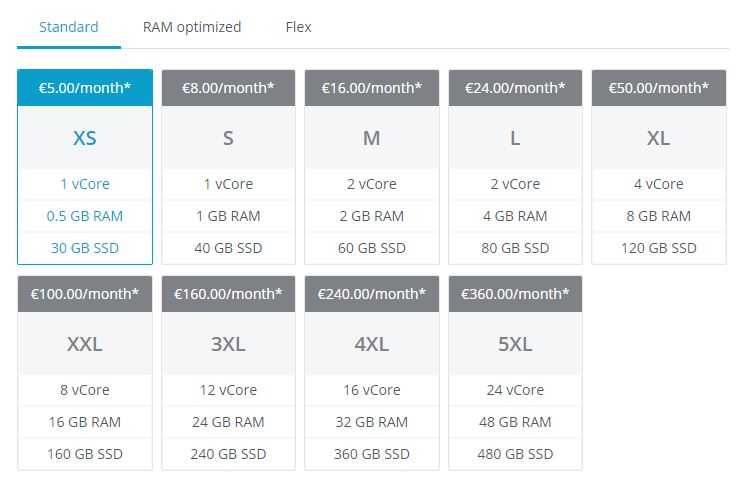
\includegraphics[width=\linewidth]{src/assets/images/vm-standard.jpg}}
    \caption{Standards VM sizes in IONOS}
    \label{fig:standard-vm-sizes}
\end{figure}

\begin{figure}[H]
    \centering
    \makebox[\textwidth]{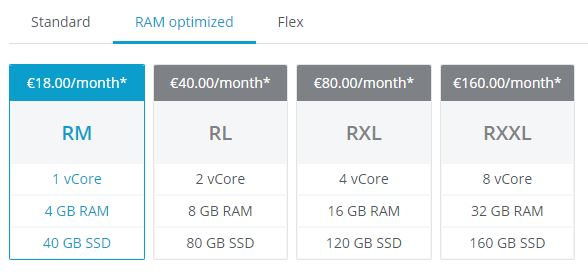
\includegraphics[width=\linewidth]{src/assets/images/vm-ram-optimized.JPG}}
    \caption{RAM Optimized VM sizes in IONOS}
    \label{fig:ram-optimized-vm-sizes}
\end{figure}

Also note that this section is only relevant in production.

% ----------------------- Software environment ----------------------- %
\section{Software environment}
This part is reserved for the presentation of the software used in the realization of the application and includes but is not limited to; programming languages, frameworks, technologies, architectures, etc...

\medskip
\textbf {For more details, see Chapter 2: State of the art}

\begin{itemize}
    \item \textbf{Git:} \newline
          \begin{minipage}{\linewidth}
              \centering
              
\includegraphics[width=2.5cm]{src/assets/logos/git_512x512.png}
              \captionof{figure}{Logo of Git}
          \end{minipage}
    \item \textbf{Docker:} \newline
          \begin{minipage}{\linewidth}
              \centering
              
\includegraphics[width=4cm]{src/assets/logos/docker_512x512.png}
              \captionof{figure}{Logo of Docker}
          \end{minipage}
    \item \textbf{Playwright:} \newline
          \begin{minipage}{\linewidth}
              \centering
              
\includegraphics[width=4.5cm]{src/assets/logos/playwright_512x512.png}
              \captionof{figure}{Logo of Playwright}
          \end{minipage}

          \newpage
    \item \textbf{NestJS:} \newline \cite{nestjs} A framework for building efficient, scalable Node.js web applications. \newline
          \begin{minipage}{\linewidth}
              \centering
              
\includegraphics[width=3.7cm]{src/assets/logos/nestjs_512x512.png}
              \captionof{figure}{Logo of NestJS}
          \end{minipage}
    \item \textbf{ReactJS:} \newline A front-end javascript library that's often used as a framework. \newline
          \begin{minipage}{\linewidth}
              \centering
              
\includegraphics[width=3.7cm]{src/assets/logos/react_512x512.png}
              \captionof{figure}{Logo of ReactJS}
          \end{minipage}
    \item \textbf{MySQL:} \newline
          \begin{minipage}{\linewidth}
              \centering
              
\includegraphics[width=5cm]{src/assets/logos/mysql.png}
              \captionof{figure}{Logo of MySQL}
          \end{minipage}

          \newpage
    \item \textbf{Sequelize:} \newline \cite{sequelize} A modern TypeScript and Node.js ORM for SQL databases. \newline
          \begin{minipage}{\linewidth}
              \centering
              
\includegraphics[width=5cm]{src/assets/logos/sequelize_512x512.png}
              \captionof{figure}{Logo of Sequelize}
          \end{minipage}
    \item \textbf{GraphQL:} \newline \cite{graphql} A query language for APIs and a runtime for fulfilling those queries with existing data. \newline
          \begin{minipage}{\linewidth}
              \centering
              
\includegraphics[width=3.7cm]{src/assets/logos/graphql_512x512.png}
              \captionof{figure}{Logo of GraphQL}
          \end{minipage}
    \item \textbf{GitLab:} \newline A DevOps software that allows secure collaboration and operations in a single application. \newline
          \begin{minipage}{\linewidth}
              \centering
              
\includegraphics[width=3.5cm]{src/assets/logos/gitlab_512x512.png}
              \captionof{figure}{Logo of GitLab}
          \end{minipage}

          \newpage
    \item \textbf{Nginx:} \newline \cite{nginx} A multi-purpose web server can also be used as reverse proxy, load balancer, mail proxy and HTTP cache. \newline
          \begin{minipage}{\linewidth}
              \centering
              
\includegraphics[width=3.4cm]{src/assets/logos/nginx_512x512.png}
              \captionof{figure}{Logo of Nginx}
          \end{minipage}
    \item \textbf{Renovate:} \newline A software that provides automatic dependency updates with support for multiple languages. \newline
          \begin{minipage}{\linewidth}
              \centering
              
\includegraphics[width=3cm]{src/assets/logos/renovate_200x200.png}
              \captionof{figure}{Logo of Renovate}
          \end{minipage}
    \item \textbf{Docker compose:} \newline A helper tool to run applications with multiple Docker containers using a .YAML format. It is often used in development. \newline
          \begin{minipage}{\linewidth}
              \centering
              
\includegraphics[width=4cm]{src/assets/logos/docker-compose_667x667.png}
              \captionof{figure}{Logo of Docker Compose}
          \end{minipage}

          \newpage
    \item \textbf{Visual Studio Code:} \newline A code editor that's used as an entire development environment with the help of extensions. \newline
          \begin{minipage}{\linewidth}
              \centering
              
\includegraphics[width=2.5cm]{src/assets/logos/vscode_512x512.png}
              \captionof{figure}{Logo of VSCode}
          \end{minipage}
    \item \textbf{Linux:} \newline A Unix-like operating system for common daily use and more commonly for servers. \newline
          \begin{minipage}{\linewidth}
              \centering
              
\includegraphics[width=3cm]{src/assets/logos/linux_512x512.png}
              \captionof{figure}{Logo of Linux}
          \end{minipage}
    \item \textbf{Make:} \newline GNU Make is used extensively throughout the application to save useful commands for the ease of maintainability. \newline
          \begin{minipage}{\linewidth}
              \centering
              
\includegraphics[width=3cm]{src/assets/logos/makefile_512x512.png}
              \captionof{figure}{Logo of Makefile}
          \end{minipage}

          \newpage
\end{itemize}

% ----------------------- Difficulties encountered ----------------------- %
\section{Difficulties encountered}
This not persay a technical difficulty as it is more of a limitation from the side of the IONOS cloud provider the organization relies on.
To have a full DevOps approach, even the infrastructure should be managed in code -also known as IAC (Infrastructure As Code)- using tools such as Terraform.
However, the cloudpanel version that we were using does not provide that functionality.
Therefore we had to scrape off the idea and simply create the virtual machines fron the UI everytime we need them.

\setcounter{secnumdepth}{0} % Set the section counter to 0 so next section is not counted in toc
% ----------------------- Conclusion ----------------------- %
\section{Conclusion}
A successfull project comes from a successfull development environment as well as a clean production environment.
For this reason, we spent quite a good amount of time setting up the infrastructure in a clean and scalable way.
